% -*- TeX-engine: luatex -*-
\documentclass[dvipsnames,presentation,aspectratio=169,14pt]{beamer}
\usepackage{hastingstheme}
\titlegraphic{
\includegraphics[scale=.35]{static_figures/du_bn.pdf}}
\author{\large Massimiliano Fasi}
\date{}


% \usepackage{template}
% \renewcommand{\authorname}{Lawrence Mitchell\inst{*}}
\renewcommand{\authoremail}{\inst{*}\texttt{lawrence.mitchell@durham.ac.uk}}

% \renewcommand{\sessionnumber}{4}
% \renewcommand{\sessiontitle}{Performance measurements}
% \usepackage{tikz}

\usepackage{pgfplots}
\pgfplotsset{compat=1.15}
\usetikzlibrary{matrix,fit,positioning,calc}
\usepackage{pgfplotstable}
\usetikzlibrary{pgfplots.groupplots}
\date{}

\begin{document}

\title{\firasemibold\color{White}%
  {\fontsize{20}{0}\selectfont SESSION 5\\
    \fontsize{40}{40}\selectfont Profiling\par}}
\titleslide

\begin{frame}
  \frametitle{Large code bases}

  \begin{challenge}{Performance counters}
    Unsuitable: too much code to annotate.

    Which section(s) of the code takes most of the time?
  \end{challenge}

  \pause

  \begin{answer}{Profiling to keep focus}
    \begin{enumerate}
    \item Find hotspots (where most time is spent)
    \item Measure performance of hotspots
    \item Optimise hotspots
    \end{enumerate}
  \end{answer}
\end{frame}

\newcommand{\gooditem}{\textcolor{Green}{\faCheck}}
\newcommand{\baditem}{\textcolor{Red}{\faTimes\,}}

\begin{frame}
  \frametitle{Profiling: types}
  \structure{Sampling}
        \begin{itemize}
        \item[\gooditem] Works with unmodified executables
        \item[\baditem] Only a statistical model of code execution
        \item[\baditem] Not very detailed for volatile metrics
        \item[\baditem] Needs long-running application
        \end{itemize}

        \vskip 5pt

        \structure{Instrumentation\vphantom{pl}}
        \begin{itemize}
        \item[\gooditem] Maximally detailed and focused
        \item[\baditem] Requires annotations in source code
        \item[\baditem] Preprocessing of source required
        \item[\baditem] Can have large \emph{overheads} for small functions.
        \end{itemize}
\end{frame}

\begin{frame}
  \frametitle{Sampling}
  \begin{columns}[c]
    \begin{column}{.4\textwidth}
      \begin{itemize}[leftmargin=10pt,itemsep=8pt]
      \item Program interrupts
      \item Periodic measurements
      \item Snapshot of the stack
      \item Potentially inaccurate
      \end{itemize}
    \end{column}
    \begin{column}{.55\textwidth}
      \begin{center}
        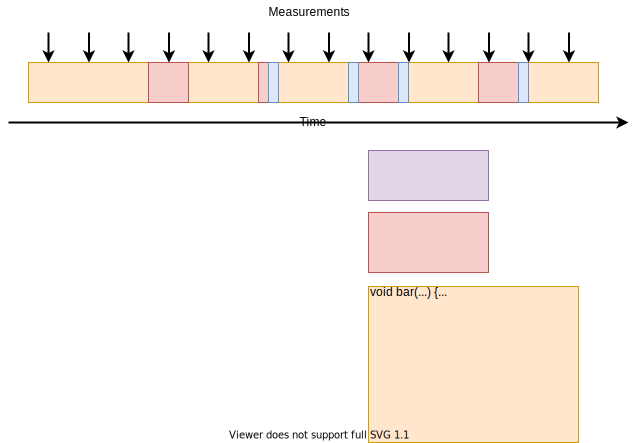
\includegraphics[height=0.7\textheight]{figures/samplingprofile.png}
      \end{center}
    \end{column}
  \end{columns}
\end{frame}

\begin{frame}
  \frametitle{Tracing}
  \begin{columns}[c]
    \begin{column}{.4\textwidth}
      \begin{itemize}[leftmargin=10pt,itemsep=8pt]
      \item Explicit measurement
      \item Extremely accurate
      \item Less information
      \item More work
      \end{itemize}
    \end{column}
    \begin{column}{.55\textwidth}
      \begin{center}
        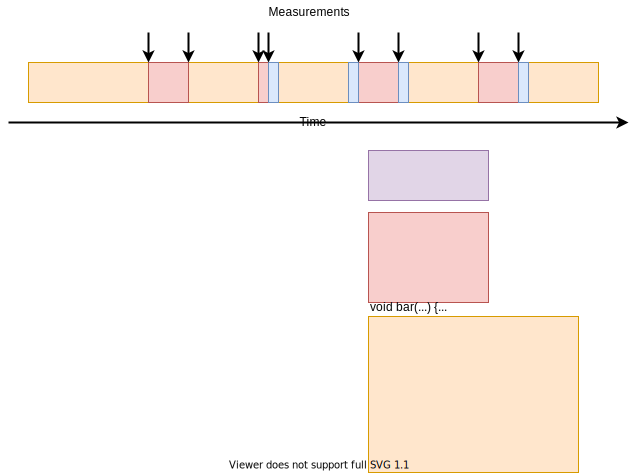
\includegraphics[height=0.7\textheight]{figures/tracingprofile.png}
      \end{center}
    \end{column}
  \end{columns}
\end{frame}

\begin{frame}[fragile]
  \frametitle{Sampling profiles with \texttt{gprof}}
  \begin{exampleblock}{Workflow}
    \begin{enumerate}[leftmargin=18pt, itemsep=10pt]
    \item Compile with profiling information and debugging symbols
\begin{minted}{bash}
gcc -pg -g <source_file> -o <executable_name>
\end{minted}
    \item Run code to produce file \texttt{gmon.out}
    \item Generate output with
\begin{minted}{bash}
gprof <executable_name> gmon.out    # flat profile and
                                    # call graph

gprof -A <executable_name> gmon.out # annotated source
\end{minted}
    \end{enumerate}
  \end{exampleblock}
\end{frame}

\begin{frame}
  \frametitle{Instrumentation \& sampling}
  \begin{itemize}[itemsep=5pt]
  \item Code is instrumented by GCC
  \item Automatic tracing of all calls
  \item Triggering of measurement is sampling based (not every call)
  \item Trade-off approach
  \end{itemize}
  \vskip 5pt

  \structure{Output}
  \begin{itemize}
  \item \emph{flat profile:} time in function, number of function calls
  \item \emph{call graph:} which function call which
  \item \emph{annotated source:} number of time each line is executed
  \end{itemize}

\end{frame}

\begin{frame}[fragile]
  \frametitle{Output: the \emph{flat profile}}
\begin{minted}[fontsize=\small]{text}
Flat profile:

Each sample counts as 0.01 seconds.
  %   cumulative   self              self     total
 time   seconds   seconds    calls   s/call   s/call  name
 99.82      5.70     5.70        2     2.85     2.85  basic_gemm
  0.18      5.71     0.01        1     0.01     0.01  zero_matrix
  0.00      5.71     0.00        3     0.00     0.00  alloc_matrix
  0.00      5.71     0.00        3     0.00     0.00  free_matrix
  0.00      5.71     0.00        2     0.00     0.00  random_matrix
  0.00      5.71     0.00        1     0.00     5.71  bench
  0.00      5.71     0.00        1     0.00     0.00  diff_time
\end{minted}
\end{frame}

\begin{frame}
  \frametitle{``Total'' and ``self'' time}
  \begin{center}
    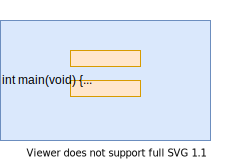
\includegraphics[width=.7\textwidth]{figures/inclusiveexclusive.png}
  \end{center}
\end{frame}

\begin{frame}[fragile]
  \frametitle{Output: the \emph{call graph}}
\begin{minted}[fontsize=\footnotesize]{text}
		     Call graph (explanation follows)

granularity: each sample hit covers 4 byte(s) for 0.18% of 5.71 seconds

index % time    self  children    called     name
                0.00    5.71       1/1           main [2]
[1]    100.0    0.00    5.71       1         bench [1]
                5.70    0.00       2/2           basic_gemm [3]
                0.01    0.00       1/1           zero_matrix [4]
                0.00    0.00       3/3           alloc_matrix [5]
                0.00    0.00       3/3           free_matrix [6]
                0.00    0.00       2/2           random_matrix [7]
                0.00    0.00       1/1           diff_time [8]
-----------------------------------------------
                                                 <spontaneous>
[2]    100.0    0.00    5.71                 main [2]
                0.00    5.71       1/1           bench [1]
\end{minted}
%   -----------------------------------------------
%                 5.70    0.00       2/2           bench [1]
% [3]     99.8    5.70    0.00       2         basic_gemm [3]
% -----------------------------------------------
%                 0.01    0.00       1/1           bench [1]
% [4]      0.2    0.01    0.00       1         zero_matrix [4]
% -----------------------------------------------
%                 0.00    0.00       3/3           bench [1]
% [5]      0.0    0.00    0.00       3         alloc_matrix [5]
% -----------------------------------------------
%                 0.00    0.00       3/3           bench [1]
% [6]      0.0    0.00    0.00       3         free_matrix [6]
% -----------------------------------------------
%                 0.00    0.00       2/2           bench [1]
% [7]      0.0    0.00    0.00       2         random_matrix [7]
% -----------------------------------------------
%                 0.00    0.00       1/1           bench [1]
% [8]      0.0    0.00    0.00       1         diff_time [8]
% -----------------------------------------------
\end{frame}

\begin{frame}[fragile]
  \frametitle{Annotated source}
\begin{minted}[fontsize=\small]{text}
     static void tiled_packed_gemm(int m, int n, int k,
                                   const double * restrict a, int lda,
                                   const double * restrict b, int ldb,
                                   double * restrict c, int ldc)
2 -> {
       const int ilim = (m / TILESIZE) * TILESIZE;
       const int jlim = (n / TILESIZE) * TILESIZE;
       const int plim = (k / TILESIZE) * TILESIZE;
       ...
     }

     static void alloc_matrix(int m, int n, double **a)
3 -> {
       ...
     }
\end{minted}
\end{frame}

\begin{frame}
  \frametitle{Optimisation workflow}
  \begin{enumerate}[itemsep=6pt]
  \item Identify hotspot functions
  \item Find relevant bit of code
  \item Determine algorithm
  \item Add instrumentation markers (see exercise)
  \item Profile with more detail/use performance models.
  \item[$\Rightarrow$] guidance for appropriate optimisation.
  \end{enumerate}
\end{frame}

\begin{frame}
  \frametitle{Exercise: finding the hotspot}
  \begin{itemize}
  \item So far, we've looked at very simple code. Now, your task will
    be to find the hotspot and do some exploration in a larger one.
  \item[$\Rightarrow$] Exercise 6 from the usual place.
  \end{itemize}
\end{frame}
\end{document}
